\chapter{Predizione con errori}
	Si è visto nel paragrafo precedente che la simulazione semplice, cioè priva di errori, ha dato ottimi risultati.\\
	Studiamo adesso la previsione dell'altezza di marea aggiungendo degli errori nella percezione che le chiocciole hanno del mondo che le circonda.\\
	\\
	Gli errori introdotti saranno quindi di due tipi: errori sulla valutazione dell'altezza della marea osservata ed errori sulla valutazione del tempo trascorso tra un'osservazione e l'altra.\\
	È plausibile pensare che queste chiocciole non abbiano una misura perfetta delle altezze di marea o del trascorrere del tempo e che facciano affidamento su una stima, più o meno accurata, di queste.\\
	Nel file relativo all'addestramento e al testing della rete neurale (Codice \ref{lst:tideLin}), e nelle simulazioni che vedremo in questo capitolo, si sono utilizzati errori relativi all'altezza di marea di massimo 0.6 (in valore assoluto, quindi tra -0.6 e 0.6), che rappresenta quindi un errore massimo del \textbf{15\%} sull'altezza di marea osservata, ed un errore relativo agli intervalli di tempo di massimo circa il \textbf{16\%}. Per quanto riguarda gli errori sulle altezze di marea, si è deciso di assegnare lo stesso errore a tutte e 5 le osservazioni successive in quanto si è supposto che, anche se la chiocciola non è sicuramente in grado di determinare l'altezza della marea con precisione assoluta, le risulterà certamente più facile capire se la marea è alzata o abbassata da un'osservazione all'altra.\\
	Nel caso si volessero cambiare tali parametri basta cambiare il valore di \textit{minTN} e \textit{maxTN}, per gli errori di altezza, e \textit{minHN} e \textit{maxHN}, per gli errori di tempo.
	\section{Predizione con errori a due ore di distanza}
		Come nel capitolo precedente, si cercherà, innanzitutto, di valutare con che errore le chiocciole riescono a predire la marea a due ore di distanza con 5 osservazioni a mezz'ora di distanza l'una dall'altra.\\
		\\
		Lo scarto quadratico medio ottenuto con questo tipo di simulazione è circa \textbf{0.124}, che corrisponde al \textbf{3.1\%} sull'altezza di marea. Questo ci dice subito che la predizione con errori di valutazione risulta essere più complessa e più difficoltosa da portare a termine.\\
		Se confrontiamo questo risultato con quello ottenuto in una previsione semplice a due ore di distanza (errore medio inferiore allo \textbf{0,0006 \%}) notiamo che l'errore è aumentato di circa un fattore \textbf{5000}. Certo un errore medio del \textit{3.1\%} rimane pur sempre un risultato ampiamente accettabile, ma questo ci fa capire come piccoli errori sui dati sensoriali possano portare ad un grandissimo aumento di complessità per la valutazione della marea futura, soprattutto per il carattere casuale che presentano tali errori: un giorno la chiocciola può sbagliarsi e vedere la marea alta 0.5 in più del normale, mentre il giorno dopo può valutarne l'altezza in modo esatto.\\
		\\
		Per riprodurre questa simulazione basta eseguire il file Codice \ref{lst:tideLin} senza apportare alcuna modifica ai parametri presenti. In questo caso un errore di massimo 5 minuti corrisponde a circa il \textit{16\%} quando l'intervallo tra due osservazioni è di mezz'ora.\\
		Di seguito alcuni grafici:\\
		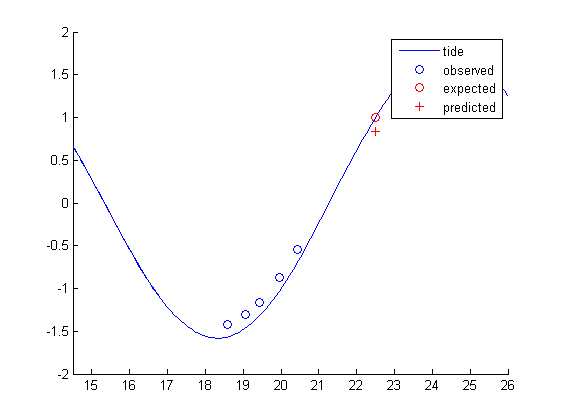
\includegraphics[width=0.6\textwidth]{error_2h_1.png}
		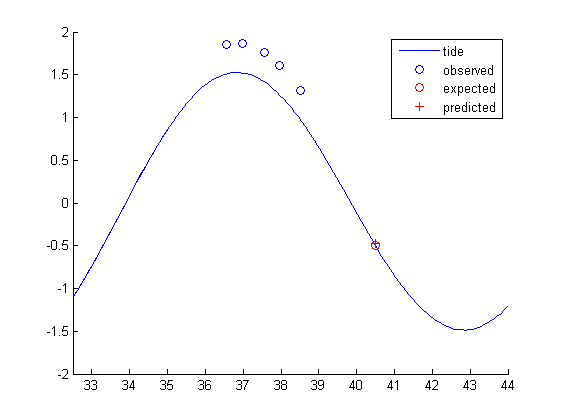
\includegraphics[width=0.6\textwidth]{error_2h_2.png}
		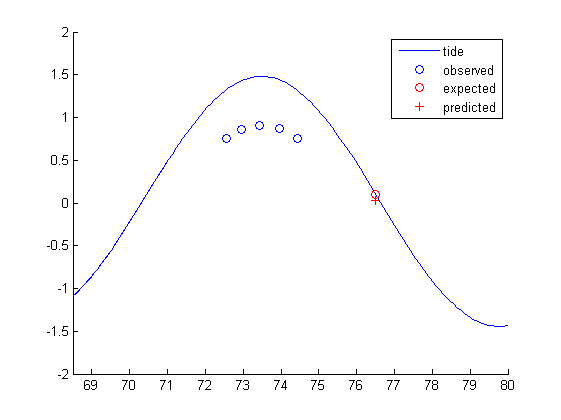
\includegraphics[width=0.6\textwidth]{error_2h_3.png}
		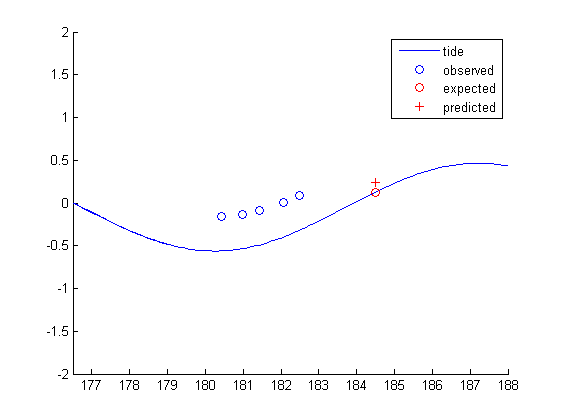
\includegraphics[width=0.6\textwidth]{error_2h_4.png}
		\FloatBarrier
	\section{Predizione con errori massima}
		Fissiamo stavolta l'obiettivo di determinare il numero massimo di ore disponibili per la predizione con un errore medio sull'altezza di marea predetta inferiore al \textit{5\%}.\\
		\\
		Sperimentalmente si è verificato che il numero massimo di ore che possono intercorrere tra l'ultima osservazione e la predizione della marea, con cinque osservazioni ogni due ore, risulta essere \textbf{28 ore}, se si vuole mantenere lo scarto quadratico medio inferiore a \textbf{0.2}, che corrisponde appunto al \textbf{5\%}.\\
		Come accennato nel capitolo precedente, se si accettano valori dell'errore medio più alti si possono ottenere molte più ore a disposizione per la previsione: ad esempio se si accetta un errore medio inferiore al \textbf{10\%} risulta che si possono fare previsioni sull'altezza di marea fino a \textbf{76 ore} dopo l'ultima osservazione. Come prima, però, un tale lasso di tempo risulta inutile alla chiocciola la quale, intuitivamente, preferisce fare una stima più accurata a breve termine piuttosto che una grossonala a distanza di giorni.\\
		\\
		Per quanto riguarda il file relativo a questa simulazione si può fare riferimento al file fin'ora menzionato (Codice \ref{lst:tideLin}), facendo attenzione a cambiare opportunamente i parametri: \textit{int} deve valere \textit{2}, \textit{forecast} deve valere \textit{28} (o \textit{76}) e \textit{minHN} e \textit{maxHN} devono valere, rispettivamente, \textit{-\sfrac{20}{60}} e \textit{+\sfrac{20}{60}} (un errore di massimo 20 minuti corrisponde a circa il \textit{16\%} quando l'intervallo tra due osservazioni è di due ore).\\
		I grafici che seguono sono relativi alla predizione \textit{28 ore} dopo:\\
		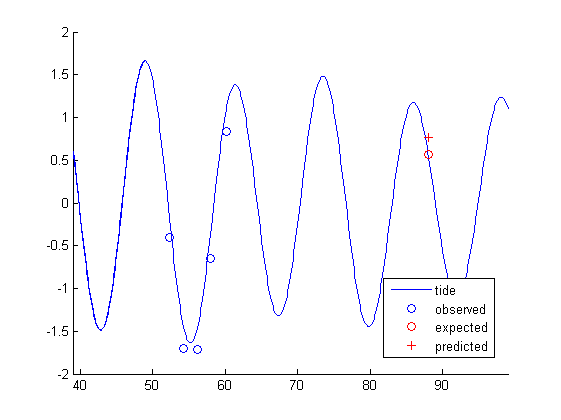
\includegraphics[width=0.6\textwidth]{error_max_1.png}
		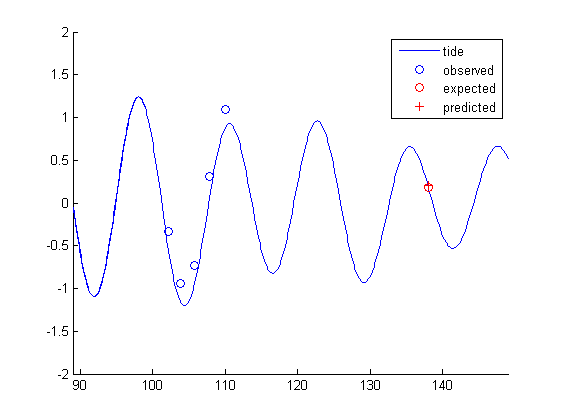
\includegraphics[width=0.6\textwidth]{error_max_2.png}
		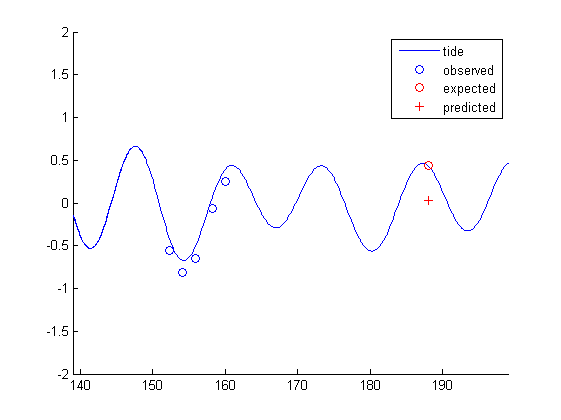
\includegraphics[width=0.6\textwidth]{error_max_3.png}
		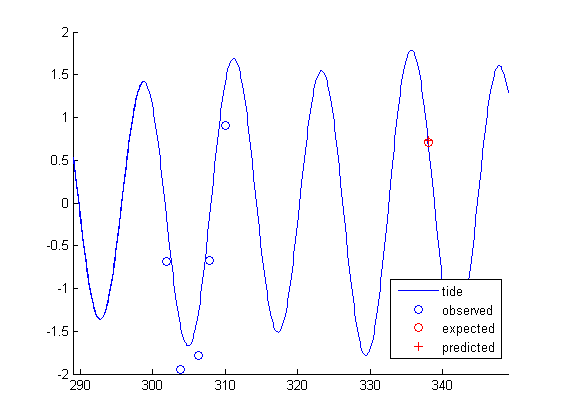
\includegraphics[width=0.6\textwidth]{error_max_4.png}
		\FloatBarrier